\chapter{Knowledge Graph Visualization Tool}
Many existing knowledge graph visualizations are restricted to displaying certain types of relationships. 
Most commonly, a class hierarchy of an ontology is visualized for the user. Other graph visualization tools are capable of visualizing data.
 A few of these graph visualizers are mentioned in \nameref{chap:Related_work}.

What we didn't find is a graph visualizer capable of displaying complex class constructs, and a few features were missing as well.
Therefore, we decided to develop our own graph visualizer, which is capable of displaying class hierarchies with complex constructs.

This chapter will present the main features of our \textit{OWLVisualizer} and explain its capabilities and limitations.

\section{Main concept}
\label{sec:MainConceps}

We decided on 3 main components that the new framework should include:
\begin{itemize}
    \item Clear Visualization: Our first goal was to facilitate navigation through the knowledge graph by highlighting the relations and classes of the graph as clearly as possible. This could be achieved, for example, by using different colors for different classes or by highlighting a class and its associated classes to which a relation exists. Additionally, we aim to make the graph as clear as possible and reduce the number of nodes to those that are ultimately essential for visualization.
    \item To clarify the relations between the queries, we implement a query builder that, given a class, can point to other classes through the relation, which in turn can point to further classes through another relation, as long as the user desires or there are no further relations. This should be done without having to use the SPARQL query language, making it much easier for the user. The Query Builder outputs a filtered graph with the selected triples.
    \item Rule Based Inference: Since a part of our work relies on inferences, we want to implement an inference query that can indicate inferred parameters based on the input of certain classes. This use case is quite specific to our scenario, but it should also be able to map to other ontologies. The output should be an action tree with the inferred parameters and a visualized graph with the associated classes that play a role in the inference.
\end{itemize}

\section{Features}

\begin{figure}[H]
    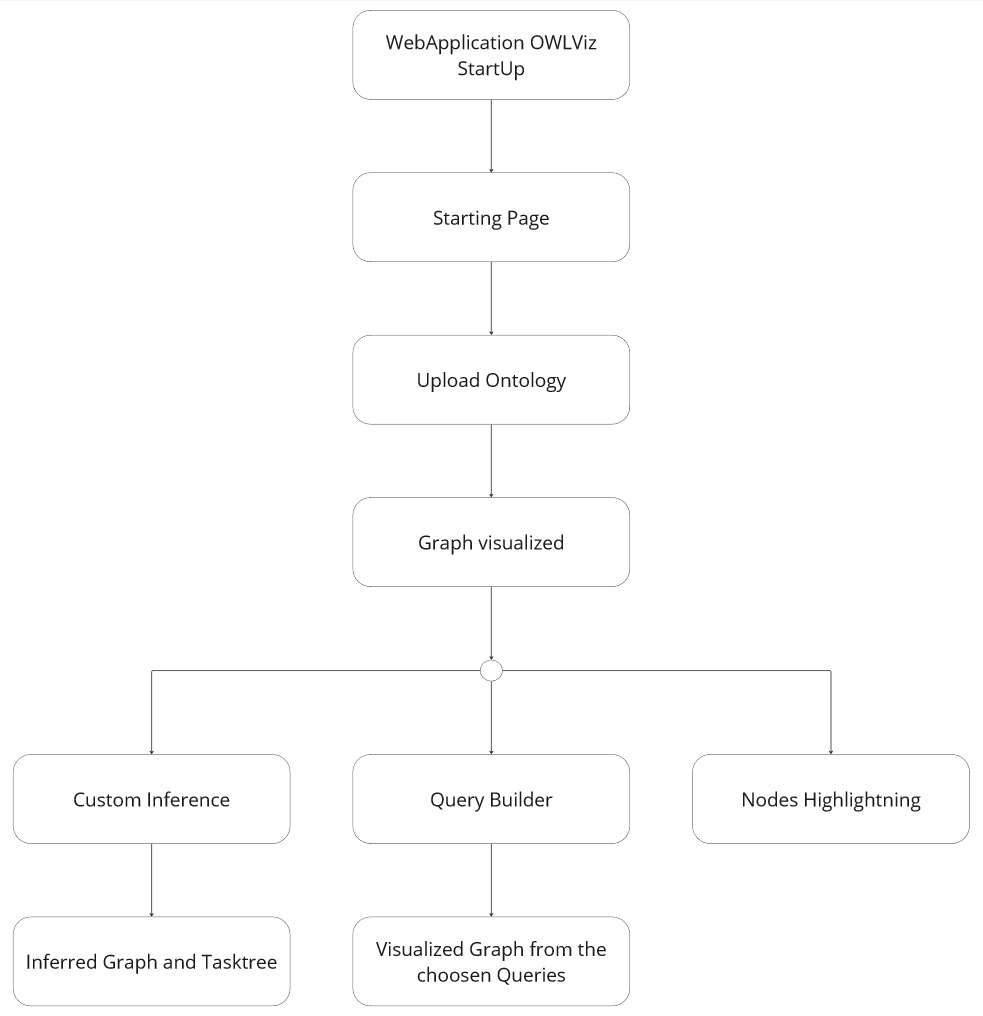
\includegraphics[scale=0.35]{Graphics/architecture_simplified.jpg}
    \label{fig:OWLViz_architecture}
    \caption{Architecture chart for the OWLVisualizer framework}
\end{figure}

\subsection{Graph Visualization}
In this section, we present a simple example of our framework, from processing the ontology to visualization in the web application. 
This is intended to facilitate the reader's understanding of our framework. 
For this purpose, we create a small and simple ontology to explain the program flow in a straightforward manner. 
Additionally, we aim to demonstrate how this ontology is processed and what the interface between the frontend and backend looks like.

The visualization library \cite{visjs} has been used to create graph visualization in web-browsers.

\begin{figure}[H]
    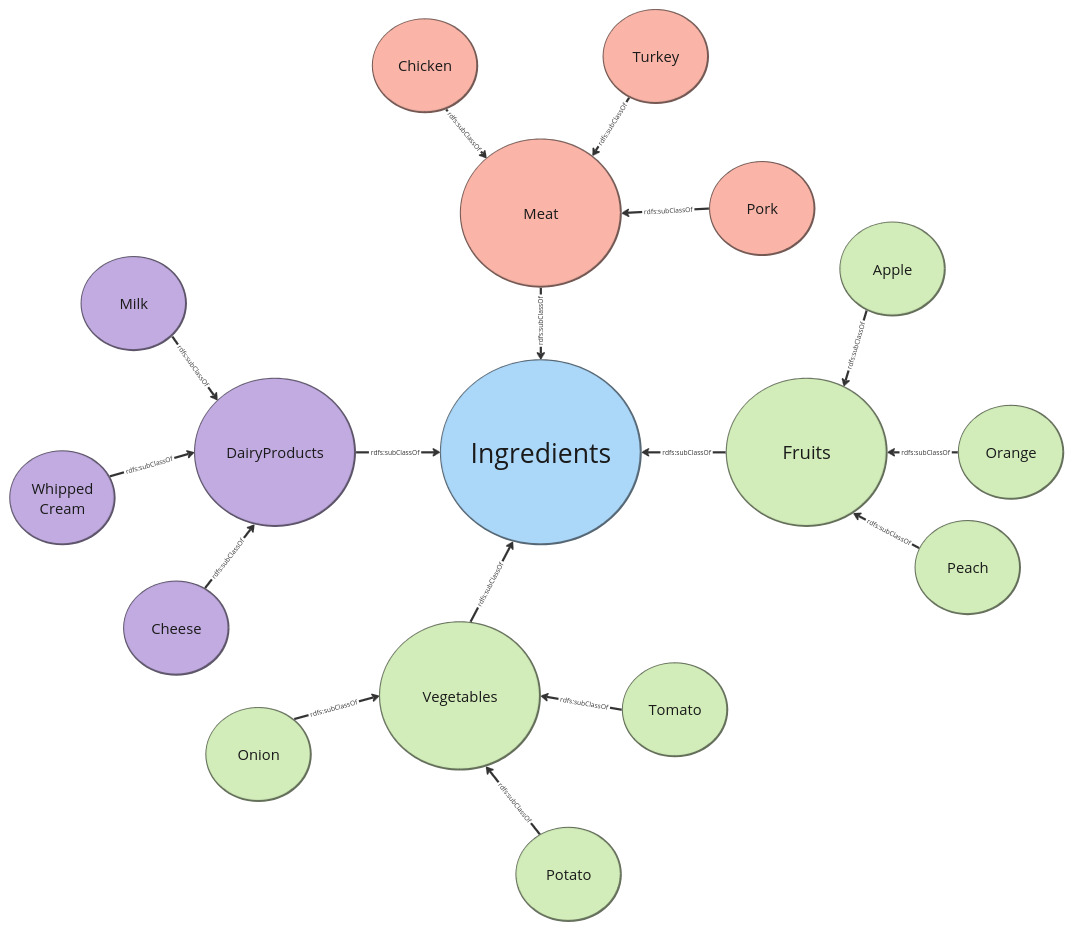
\includegraphics[scale=0.4]{Graphics/simple_ontology.jpg}
    \caption{Trivial example of an ontology}
\end{figure}
    
The ontology created for this purpose aims to provide a simple representation of various animal species. It includes superclass categories such as \textit{Fruits, Vegetables, Meat, and Dairy Products}, as well as subclasses like \textit{Apple} and \textit{Orange}, which are subclasses of the \textit{Fruits} superclass. This ontology does not depict complicated relations; rather, the individual classes are only connected to each other through the \textit{subClassOf} relation.

\subsection{Graph Processing}
The core component of the graph visualizer is the visualization of a hierarchy of classes. In this hierarchy, two nodes are connected by a directed edge, 
where the source node is the child node and the target node is the parent node. All edges are labeled either as \textit{subClassOf} or \textit{equivalentClass}.

To create the visualization from the graph, the ontology is parsed, and a triple matching process is applied to identify 
all classes that use \textit{subClassOf} or \textit{equivalentClass} as predicates.

By default, all nodes are uniformly colored green. However, in the \textit{mixing} and \textit{FoodCutting} ontologies, 
additional colors are used to highlight differences.
\begin{figure}[H]
    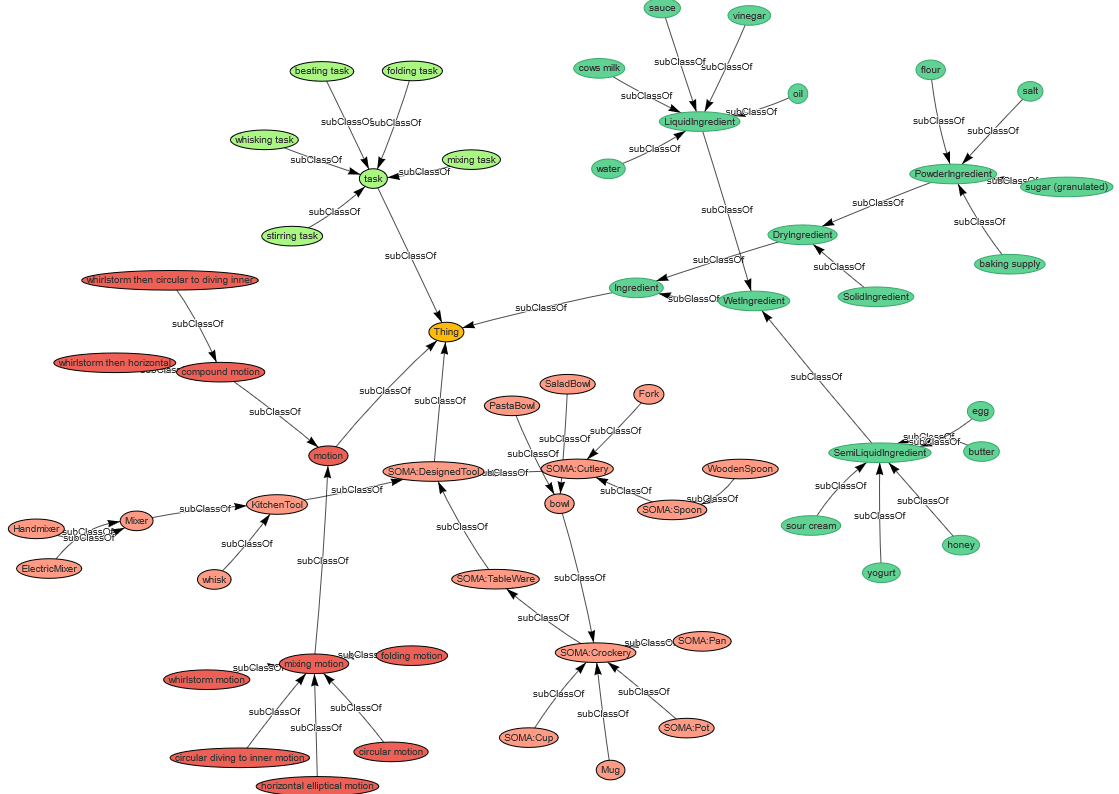
\includegraphics[scale=0.5]{Graphics/OwlVisualizer/graphProcessing1.png}
    \centering
    \caption{Processed Class Hierarchy}
\end{figure}

The graph visualizer is also capable of visualizing complex class expressions. 
However, it is essential to understand why the parsed expressions should not be used directly, as illustrated in figure \ref{fig:graphProcessing2}. 
Blank nodes and meta information associated with these expressions are generally useless to the user. 
This type of visualization is not compact, and users unfamiliar with ontology parsing will find it confusing and uninformative. 
Additionally, visualizing each parsed node increases the number of nodes and edges, which degrades performance. 
Therefore, a more compact visualization of complex restrictions is necessary to ensure clarity and maintain optimal performance.

\begin{figure}[H]
    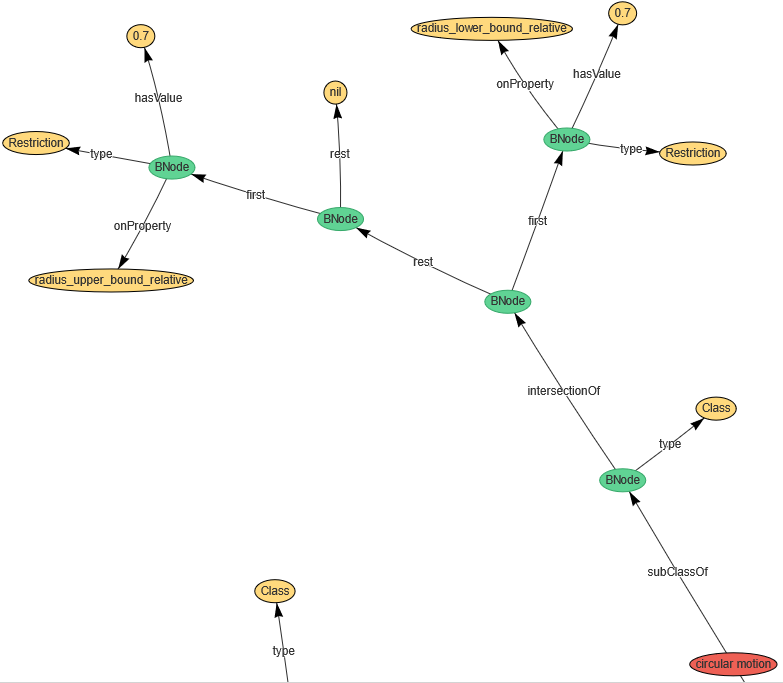
\includegraphics[scale=0.5]{Graphics/OwlVisualizer/graphProcessing2.png}
    \centering
    \caption{Visualize parsed class restrictions}
    \label{fig:graphProcessing2}
\end{figure}

To achieve a compact representation of class expressions, we recursively traverse the parsed class expression, 
searching for essential information such as the relations used and their corresponding values. 
All blank nodes are implicitly skipped and not visualized. Additionally, meta information is excluded.

The visualizer can also handle nested expressions, as well as intersections and unions. Each \textbf{AND} node indicates that all connected elements belong to the intersection.
Similarly, each \textbf{OR} node indicates that all connected elements belong to the union.

In the figure \ref{fig:graphProcessing3}, the following expression is visualized:

CircularMotion \textit{subClassOf} (radius upper bound relative value 0.7) and (radius lower bound relative value 0.7)

\begin{figure}[H]
    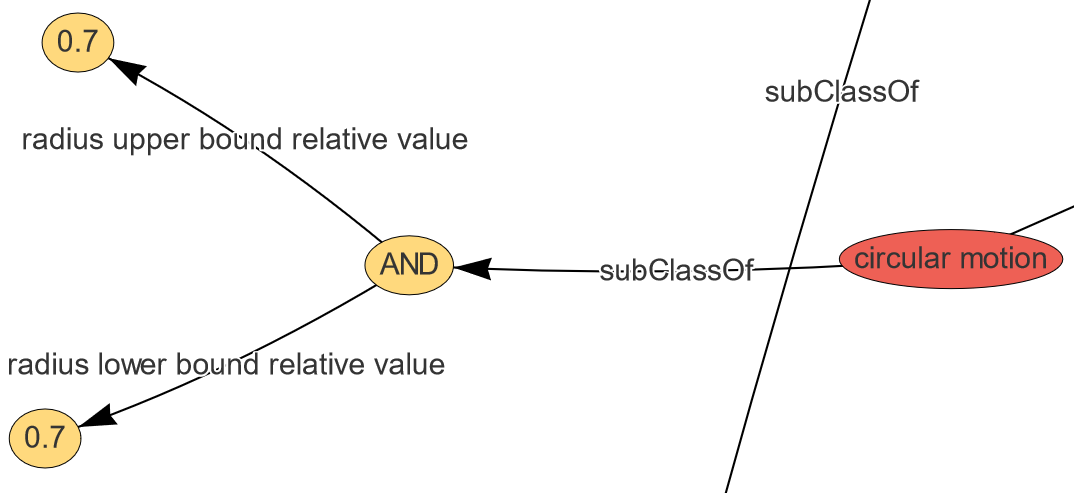
\includegraphics[scale=0.3]{Graphics/OwlVisualizer/graphProcessing3.png}
    \centering
    \caption{Visualize parsed class restrictions}
    \label{fig:graphProcessing3}
\end{figure}

\subsection{Load Ontology}

By pressing the \textit{Load Ontology} button, users can load a wide range of ontologies that have the \textit{.owl} file extension.
Upon selecting the ontology, the \textit{OwlVisualizer} begins parsing the ontology to process the ontology. 
Once the processing is complete, a visual representation of the ontology is created, which can be explored by the users freely. 


\begin{figure}[H]
    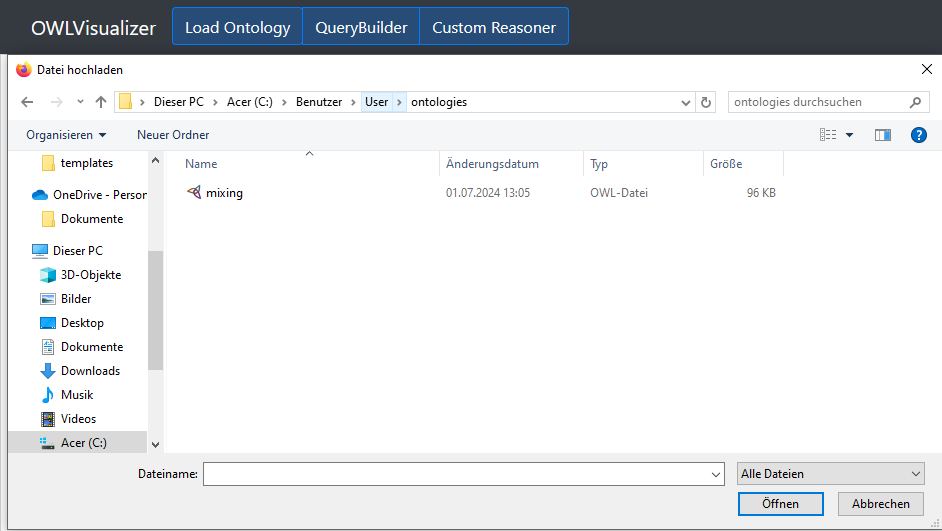
\includegraphics[scale=0.35]{Graphics/OwlVisualizer/loadOntology1.png}
    \centering
    \caption{Loading Ontology}
    \label{fig:loadOntology1}
\end{figure}

Attempting to load any other file types results in an error message being displayed on the website. 
When a user tries to upload a file that does not have the \textit{.owl} extension, the \textit{OWLVisualizer} notifies 
the user that the file extension is not supported by this tool, via an error message. 

\begin{figure}[H]
    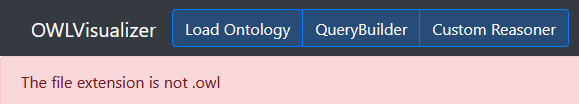
\includegraphics[scale=0.5]{Graphics/OwlVisualizer/loadOntology2.png}
    \centering
    \caption{\textbf{Error}: Unsupported File Type}
    \label{fig:loadOntology2}
\end{figure}

Additionally, if an ontology can't be parsed, an error message is thrown that ontology couldn't be
loaded properly. Whenever this issue is encountered during the parsing of the selected ontology, it immediately stops and triggers an error notification. 
This message informs the user that there was a problem with loading the ontology, possibly due to a formatting error or an unsupported structure within the file. 
This error message informs the user of this particular issue; the \textit{OWLVisualizer} doesn't attempt to deal with this problem.

\begin{figure}[H]
    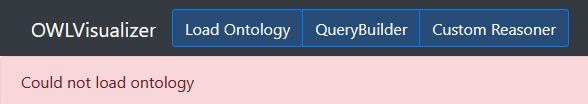
\includegraphics[scale=0.5]{Graphics/OwlVisualizer/loadOntology3.png}
    \centering
    \caption{\textbf{Error}: Ontology Load Failure}
    \label{fig:loadOntology3}
\end{figure}

\subsection{Search Classes}
The \textit{OwlVisualizer} includes a feature that suggests classes, which are visualized as nodes, 
for users to focus on, improving their ability to navigate and understand complex networks.

\begin{figure}[H]
    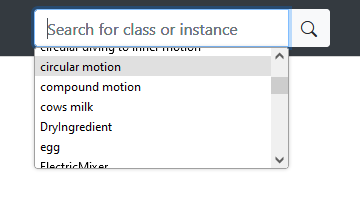
\includegraphics[scale=0.6]{Graphics/OwlVisualizer/searchClass1.png}
    \centering
    \caption{Search bar suggesting available classes}
\end{figure}

The key implementation for this feature is a search bar that suggests all visualized classes. 
Any nodes belonging to a class restriction are not suggested. 
The available suggestions are sorted in descending order, allowing users to easily search
for classes and explore the class hierarchy without assuming prior familiarity with the ontology.

\begin{figure}[H]
    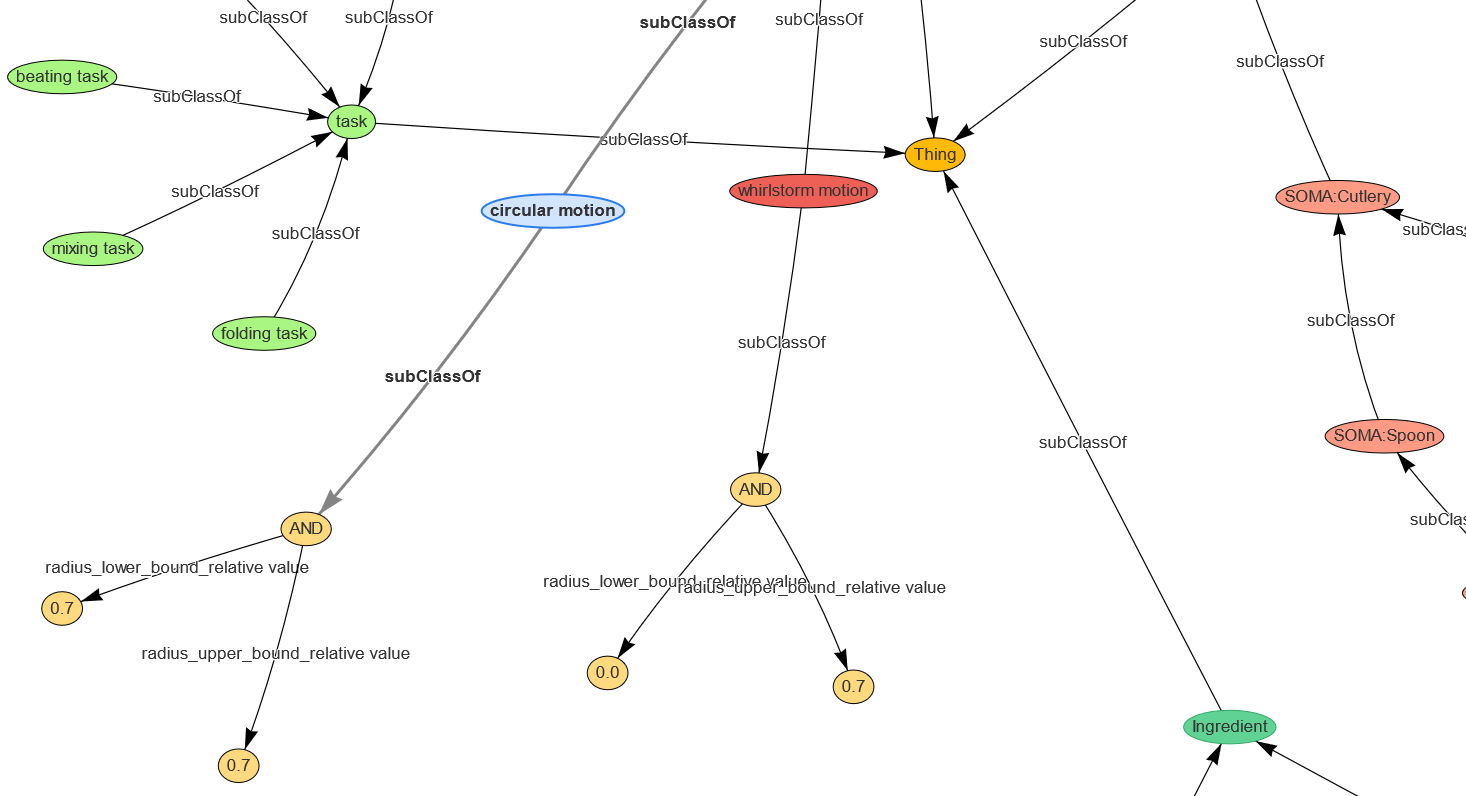
\includegraphics[scale=0.25]{Graphics/OwlVisualizer/searchClass2.png}
    \centering
    \caption{Focus node}
\end{figure}

Users can press Enter inside the search bar or click the search button to immediately focus on the chosen class. 
Focusing on the class is achieved by zooming to the respective node and highlighting it. 
This allows users to quickly identify the corresponding node along with all of its parent and child nodes.

\subsection{Custom Inference - Mixing}

One option for the user to execute functions on a graph is the Inference Builder. 
It's important to note that the Custom Inference Builder is not a generic use case and in this version, it's tailored to the Mixing Graph (see \nameref{chap:Data_representation}). 
In our case, we infer a motion and its corresponding parameters based on a given task and a list of ingredients. 
\begin{figure}[H]
    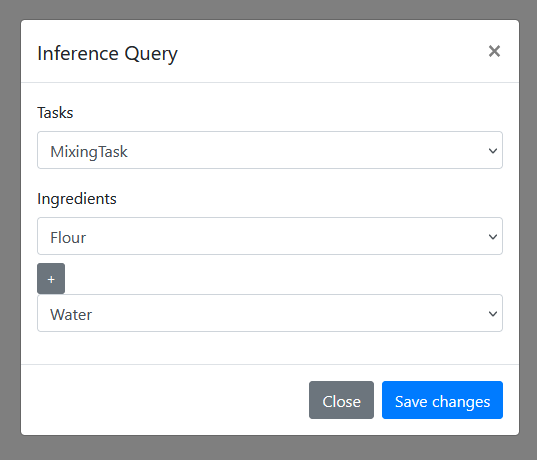
\includegraphics[scale=0.45]{Graphics/inference_user_input.png}
    \caption{Select fields for the inference.}
\end{figure}
The Custom Inference Builder then generates a graph that only displays the corresponding nodes for clarity, as well as a task tree that can be followed by an agent.
In the first step, the task and the ingredients are sent to the backend for inference, which in turn sends back the inferred motion and parameters to the frontend.
The backend function processes the inference with the received parameters, which results in a task tree as well as a filtered graph, that contains only the classes that are used in the inference, these are then used for visualization.
In the frontend, the data is processed using an \textit{AJAX} request. After sending the task and the list of ingredients, the response, which includes the generated graph and task tree, is returned to the frontend and processed. A \textit{JavaScript}-function then creates a graph with the nodes and edges received from the backend and generates a table with a variable number of rows based on the backend's output.
After processing the data, the graph and the task tree are visualized based on the user input.

\begin{figure}[H]
    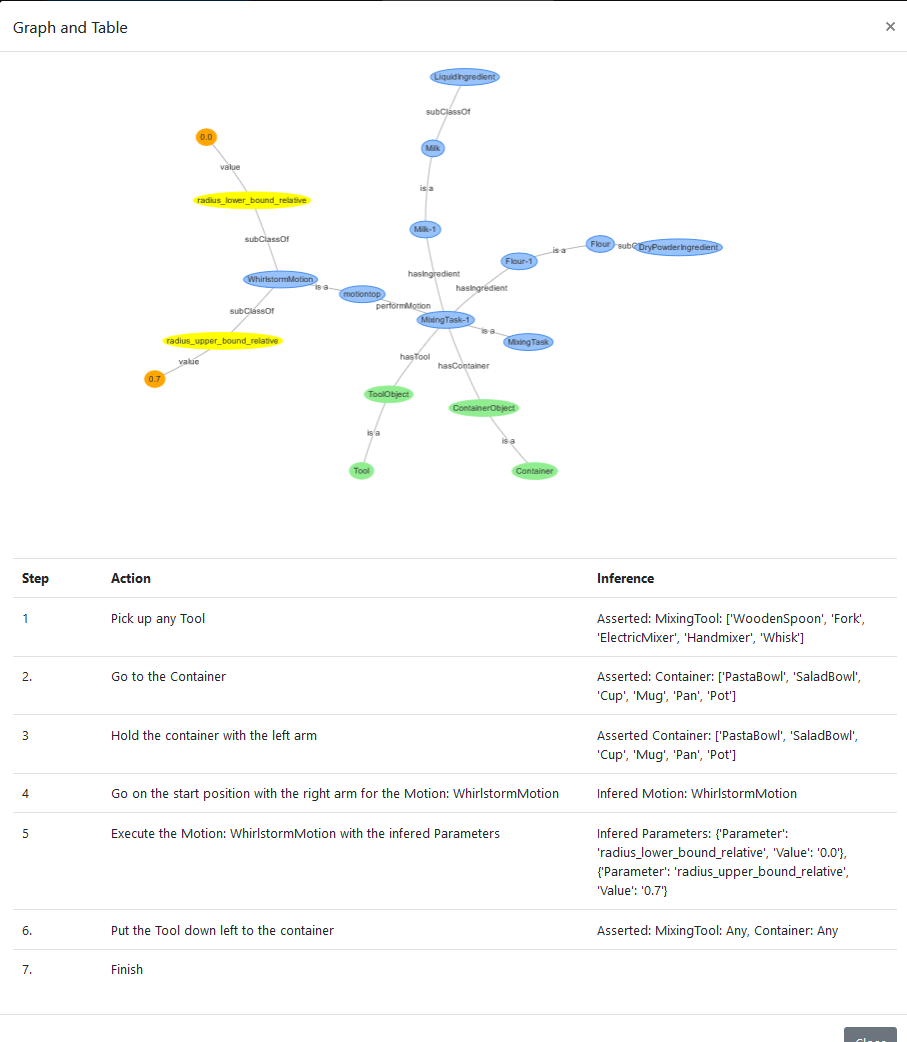
\includegraphics[scale=0.5]{Graphics/new_inference_graph.png}
    \caption{inferred graph and task tree.}
    \label{fig:graph_inferred}
\end{figure}

The data processing and the detailed implementation of the Inference Builder will be further explained in the \nameref{sec:Implementation} section.
\subsection{QueryBuilder}

\section{Implementation}
\label{sec:Implementation}

This section explains the detailed implementation of the framework and highlights the challenges and solutions encountered during implementation. In the previous section, we provided a trivial example intended to serve as an introduction for users to understand the framework's basics. However, since ontologies can vary in structure and some relations can be complex, a simple implementation may not suffice in most cases.

We will begin by explaining the implementation of the backend, and towards the end of the section, we will also address some aspects of the frontend. In the conclusion, we will touch upon points that, in our opinion, could be implemented in the future and discuss any problems/limitations this framework might have.
\subsection{BackEnd}

As explained in the \nameref{sec:Architecture} section and demonstrated in the Introductory Example section (see: \nameref{sec:Introducing the framework with a trivial example}), the framework uses \textit{flask} (see \ref{sec:flask}) as its backend interface. 
This ultimately serves to send processed data to the frontend or receive data from it. Now, we'd like to explain how this data is processed and how it has been adequately prepared.
\subsubsection{Graph Verarbeitung - Work in Progress}

To visualize a graph using the JavaScript library \textit{vis.js} (NOTE), we need a set of nodes and edges. An example of how these could be processed was explained here (NOTE). The existing classes of an ontology are not always connected only by the \textit{subClassOf} relation. Some relations pose challenges in the graph because lists of possible classes related to a superclass can also appear. This poses a problem for visualization because in such cases, so-called \textit{Blank Nodes} appear. These nodes do not represent any information but merely serve as connection nodes between 2 or more classes. These nodes are connected by relations such as \textit{owl:intersectionOf}, \textit{owl:first}, or \textit{owl:rest} and have no added value for our visualization. The first challenge was to adequately process these nodes to remove \textit{Blank Nodes} from the visualized graph and to represent the correct relation between the classes between which these \textit{Blank Nodes} existed

\subsubsection{Implementation of the Query Builder - Work in Progress}


\subsubsection{Implementation of the Inference Builder}
As described in the \nameref{sec:Architecture}, the Inference Builder is intended to visualize and organize the results of inference within the ontology. 
The inference refers to defined \textit{SWRL} rules (see: \nameref{sec:SWRL}), which can then be queried using the \textit{OWLReady2} library (see: \nameref{sec:OWLReady}).
Therefore, the implementation assumes this type of rules. The rules implemented by us were explained in the \nameref{chap:Motions} chapter. 
Ultimately, the goal is to execute the inference based on user input and visualize the results.
\paragraph{User Input}

The user selects a task and any number of ingredients.
\begin{figure}[H]
    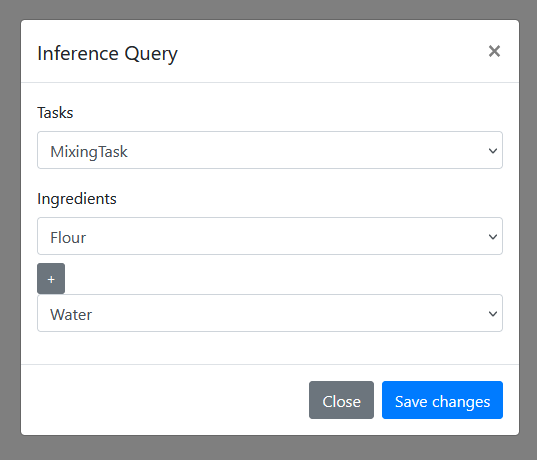
\includegraphics[scale=0.45]{Graphics/inference_user_input.png}
    \caption{Select fields for the inference.}
\end{figure}
These data are extracted from the ontology using the \textit{rdfLib}(see  
\ref{sec:RDFLib}). In the following it will be explained further.

\begin{lstlisting}[caption={Task and ingredient extraction},captionpos=b]
   def get_tasks():
        iterate over classes that are related by rdfs:subClassOf
        check for subclasses of Task and appent to task_list
        return task_list

    def get_ingredients():
        analogously to get_tasks()
        filter for ingredients that are only subclasses.
        return ingredients_list


\end{lstlisting}


\begin{itemize}
    \item Each triple where the predicate of the relation matches \textit{subClassOf} is queried. Additionally, it checks whether the object corresponds to the class \textit{Task}. These elements are then added to a list, which is also returned.
    \item Similar to the \textit{get\_task()} function, the subclasses of ingredients are returned. The only difference is that the function is called recursively since the class \textit{Ingredients} has subclasses at multiple levels. Therefore, it also checks which class has no more subclasses.
\end{itemize}

These data can be sent to the frontend by calling the corresponding \textit{@app.route}

\begin{lstlisting}[caption={Sending task and ingredients list to the frontend},captionpos=b]
    @app.route('/task_ingredients')
    def get_tasks_and_ingredients():
        return {tasks: get_tasks(), 
            ingredients: get_ingredients()} 

\end{lstlisting}

The previously described functions are called, and the data is sent to the frontend in \textit{JSON} format. In the frontend, this data is fetched and processed.

\begin{lstlisting}[caption={Fetch and populate select fields},captionpos=b]
    function ($) {
        url: '/task_ingredients'
        success: function(data)
        {
            taskSelect = #taskSelectElement
            iterate through the list of tasks
            appent each task as an option to the taskSelectField
        }
        {
            analogously for ingredients
        }
    }

\end{lstlisting}



This function populates the entries of the select fields for task and ingredient selection with the data from the backend. 
By doing so dynamically, it ensures that even if the ontology has new entries in these classes, they will always be available for the user's selection.

\paragraph{Inference}
\label{par:Inference}

An example can illustrate the process of inference calculation. Taking the above example (see: \ref{fig:graph_inferred}), we have the input task: \textit{MixingTask} and the ingredients: \textit{Flour} and \textit{Water}. 
These two ingredients correspond to the superclasses \textit{PowderIngredient} and \textit{LiquidIngredient}, respectively (see: \nameref{chap:Data_representation} for more information 
about the structure of the ontology.). This combination ultimately corresponds to the \nameref{sec:SWRL}-Rule:
\begin{lstlisting}
MixingTask(?x) ^ PowderIngredient(?ing1) ^ hasIngredient(?x, ?ing1)
^ LiquidIngredient(?ing2) ^ hasIngredient(?x, ?ing2) ^ Motion(?motion) 
^ performMotion(?x, ?motion) -> WhirlstormMotion(?motion)
\end{lstlisting}

From this, the motion \textit{WhirlstormMotion} is inferred with the corresponding parameters:
\begin{lstlisting}
    radius_lower_bound_relative  0.0
    radius_upper_bound_relative  0.7
\end{lstlisting}
To calculate this inference, we use the library \textit{OWLReady2} (see: \nameref{sec:OWLReady}), which enables us to utilize a reasoner for the inference.

\begin{lstlisting}[caption={Inference},captionpos=b]
    def get_inference(task, ingredients):
        load the ontology
        initialize a task instance
        iterate over the list of ingredients
            initialize an instance for every ingredient
            relate the ingredients to the task instance
        
        initialize the motion
        relate the motion to the task instance

        extract the rules from the ontology

        start the reasoner
        infer the motion and parameters based on the task 
        and ingredients input

        return motion, parameters


\end{lstlisting}
\begin{itemize}
    \item The classes are instantiated. The function takes parameters \textit{task}, corresponding to a task, and \textit{ingredients}, corresponding to a list of ingredients. The ontology for the \textit{OWLReady2} library is instantiated to utilize the reasoner. Next the \textit{task} is instantiated, since the task comes as input in the full \textit{IRI} format, it needs to be processed first. The same is done analogously for the ingredients, this time only for a list of ingredients. Subsequently, the instances of the \textit{ingredients} are added to the instance of \textit{task}.
    \item A top-level \textit{Motion} is instantiated to indicate that the \textit{Motion} is inferred during reasoning.
    \item The existing rules are examined and matched with the input to infer the correct \textit{SWRL} rules.
    \item Lastly, the reasoner is executed. The inferred motion is stored, and now it is about determining the required parameters based on the motion. These parameters are then stored in a dictionary. The function returns the motion and the parameters.
\end{itemize}

\paragraph{Preparing the Output}
For clarity, we have decided to reduce the graph to only the classes used in the inference. The middle node of the graph represents the task instance selected by the user. 
From this node, you can reach the other classes that are important for the inference. 
These classes correspond to the classes of the ingredients, i.e., the ingredient instances selected by the user, the inferred motion along with parameters, 
and each instance for the tools and containers, each of which can represent any possible combination if no selection has been made.
\begin{lstlisting}[caption={generating the graph},captionpos=b]
    def generate_task_tree_and_graph_data(task, ingredients):
        motions, parameters = get_inference(task, ingredients)

        initialize a graph
        process through the inlcuded classes in the inference 
        and add them to a set.
        append the elements of this set to the graph and 
        inlcude the edges by considering the corresponding 
        relations
        process the inferred parameters

\end{lstlisting}

\begin{itemize}
    \item The results of the inference function (see: \nameref{par:Inference}) are stored and used for further processing.
    \item We initialize an empty graph, which will be filled with nodes and edges throughout the function. Additionally, a set is initialized for the set of nodes.
    \item Based on the task instance, the graph is structured starting from this node. It checks which relations exist for this instance and accordingly inserts into the set of edges and nodes. Additionally, for the \textit{hasIngredient} relation, the superclass of the ingredient is considered. Finally, the edge labeling is chosen based on the relation, and the classes are added to the graph.
    \item Iterating over the set of nodes, they are added to the graph.
    \item The inferred parameters are processed and added to the graph in the end.
\end{itemize}

For the task tree, we create a 3-column table. The first column represents the step, the second column represents the action, and the third column represents the parameters used to illustrate them. The task tree is a list of entries, which can also contain dynamic data such as motions and ingredients.

\begin{itemize}
    \item 1: The first entry pertains to the robot's action, which is to choose a tool for the upcoming actions. The list of \textit{Tools} corresponds to the subclasses of \textit{Tools} from the ontology. (REFERENCE TO GET TOOLS LEAF)
    \item 2 and 3: Analogous to the first entry, the container is chosen and must be held with an arm for the upcoming motion.
    \item 4: This action describes the starting point of the motion; each motion has its own starting point (see: \nameref{chap:Motions}).
    \item 5: In this step, it is explained with which parameters the motion must be executed.
    \item 6: Once the motion execution is complete, the used tool is set aside.
    \item 7: The final step does nothing but announce the end of the task tree.
    \end{itemize}

These data are forwarded to the frontend via the \textit{flask} interface, where ultimately the graph and the task tree are visualized (see: \ref{fig:graph_inferred})

\section{Fazit}

\subsection{Weaknesses}

\paragraph{Using vis.js}
Using the graph visualization library vis.js yields poor performance on large graphs.
This reason is known to the developers of vis.js (See reference) and the cause of the problem is coming
from the physics simulation. The visualized graph is a force directed graph and the physics simulation attempts to make a user readable graph 
by seperating and clustering nodes who don't or belong to each other. This is done iteratively and consumes a lot of time for large sets of nodes
connected via many edges. The more interconnected the graph is the more terrible the performance gets. 

\paragraph{Data Visualizer}
This framework in its core is not a graph data visualizer. While it is absolutely able to display relationships and attributes of instance data, visualizing 
large datasets defined as ontology is not feasible. It is limited by vis.js which is poorly optimised for large sets of nodes and edges. 
Thus this framework can't be a graph data visualizer. 